\chapter{Brugervejledning}
OBS: Som programmets opbygning lige nu gøres der opmærksom på at der mangler nogle funktionaliteter. \\
Hvis der er problemer med at forbinde til databaseserveren, kan oplysninger omkring forbindelsen findes ved at gå ind under:\\ 
\\
NetBeans projektet “MMMI\textbackslash src\textbackslash mmmi\textbackslash Data\_ layer\textbackslash Connection.java”.\\
Under denne klasse kan variablerne url, username og password findes:\\
String url = "jdbc:postgresql://mmmihosting.ddns.net:3306/mmmidb";\\
String username = "pi";\\
String password = "MMMI\_ pi\_ server";\\
\\
Når man skal til at benytte programmet vil du blive mødt af en login vidnue. Dette vindue er et login til selve MMMI systemet. Du skal dermed indtaste brugernavn og adgangskode og trykke herefter på knappen ”login”. (se figur \ref{bru:f1})\\
\begin{center}
\begin{figure}[h]
  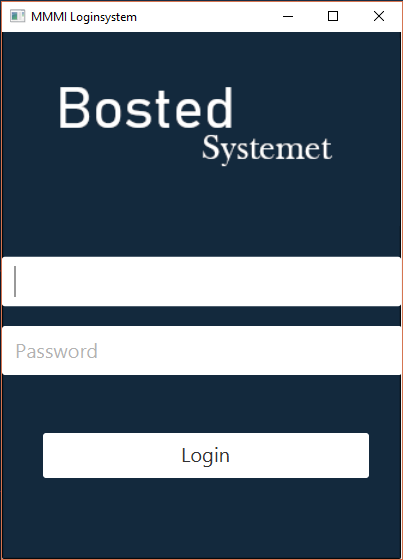
\includegraphics[scale=0.3]{./PNG/brugervejledning/figur1.PNG} 
  \caption{}
  \label{bru:f1}
\end{figure}
\end{center}
\begin{figure}[h]
  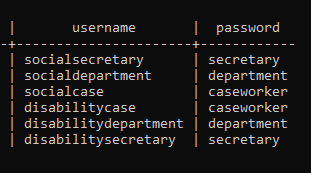
\includegraphics[scale=1]{./PNG/brugervejledning/loginInfo.PNG} 
  \caption{Viser hvad der kan bruges til at logge ind}  
  \label{bru:login}
\end{figure}
\newpage
\textbf{Overordnet konto til test:}
Når du har trykket på loginknappen, vil du blive viderestillet til hovedprogrammet MMMI. MMMI er designet til at være et sagsforløb program til at hjælpe sagsbehandlere med at løse sagsopgaver. 
Når du er logget ind får du vist følgende vindue, se figur \ref{bru:f2}. 
\begin{figure}[htb!]
  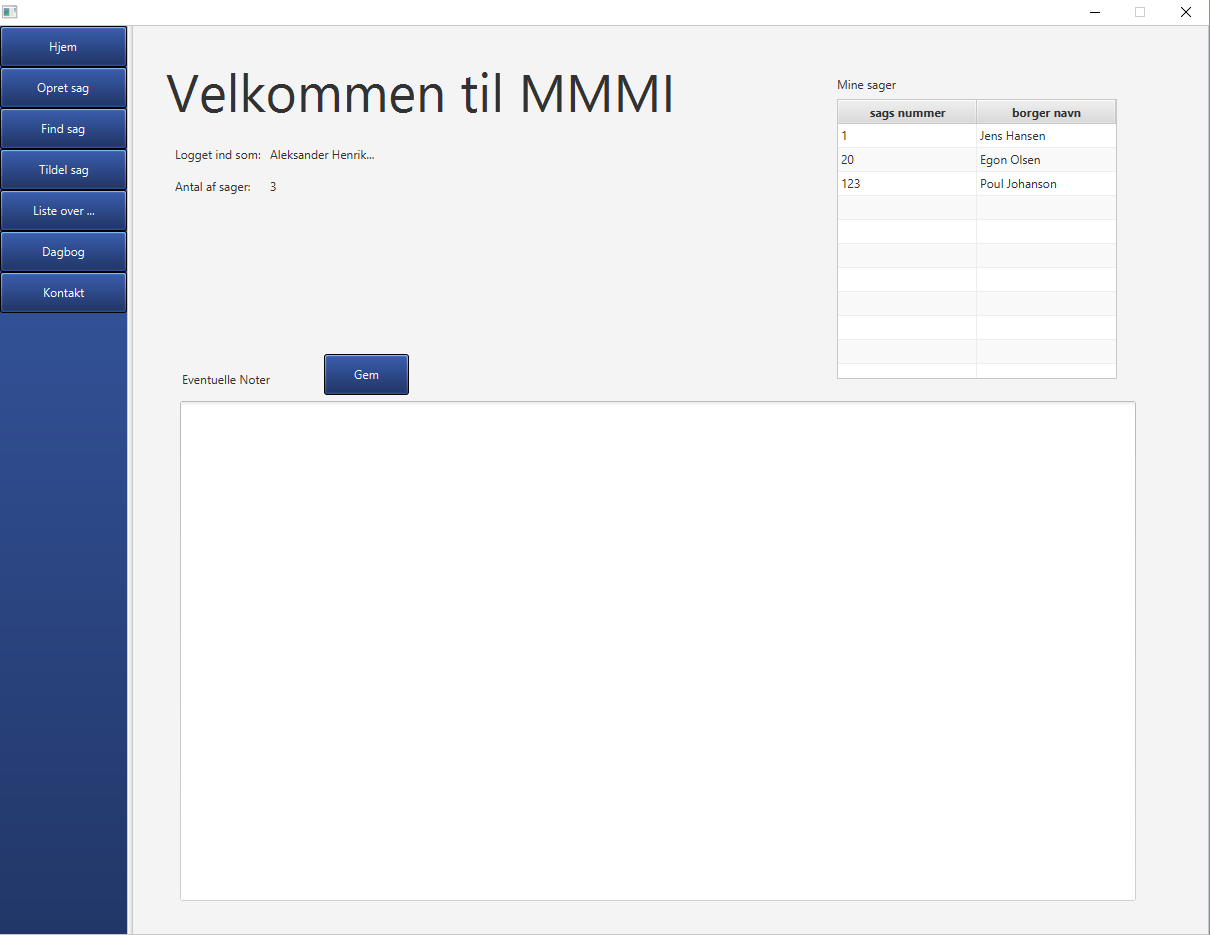
\includegraphics[width = \linewidth]{./PNG/brugervejledning/figur2.PNG} 
  \caption{}  
  \label{bru:f2}
\end{figure}
\newpage
Når du er logget ind får du vist ”hjem” fanen hvor der kan ses hvem du er logget ind som, antal sager og hvilke sager man har i højre side (figur 2). I tekstfeltet under ”gem” knappen kan der skrives en note til en sag ved at markere sagen i sagsdisplayet, se figur \ref{bru:f3}. 
\begin{figure}[htb!]
  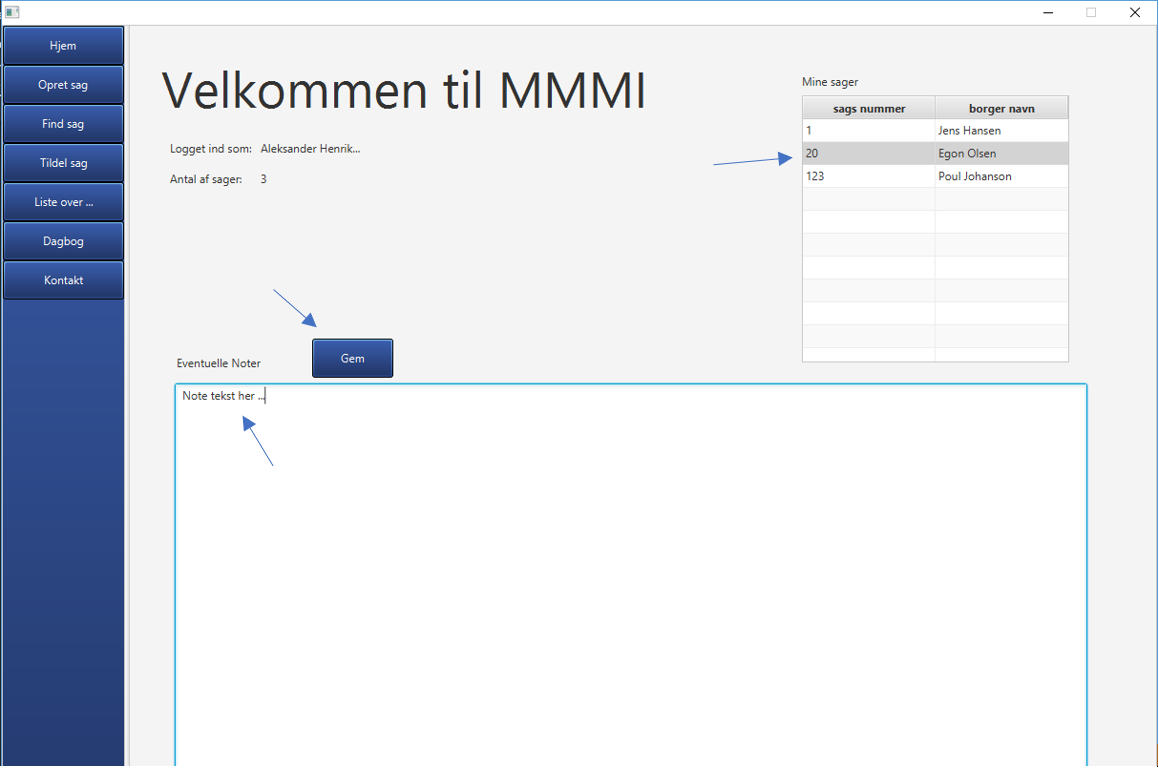
\includegraphics[width = \linewidth]{./PNG/brugervejledning/figur3.PNG} 
  \caption{}  
  \label{bru:f3}
\end{figure}
\newpage
Når der trykkes på opret sag, vil der blive vist en sagsåbningsformular som kan udfyldes. I sagsåbningsformularen skal henvendelsesfeltet udfyldes før en sag kan gemmes. Det er vigtigt at den lille ”gem knappen” i dokumentet skal klikkes på først, før man fortsætter, så de ting der er udfyldt gemmes. (se figur \ref{bru:f4})
\begin{figure}[htb!]
  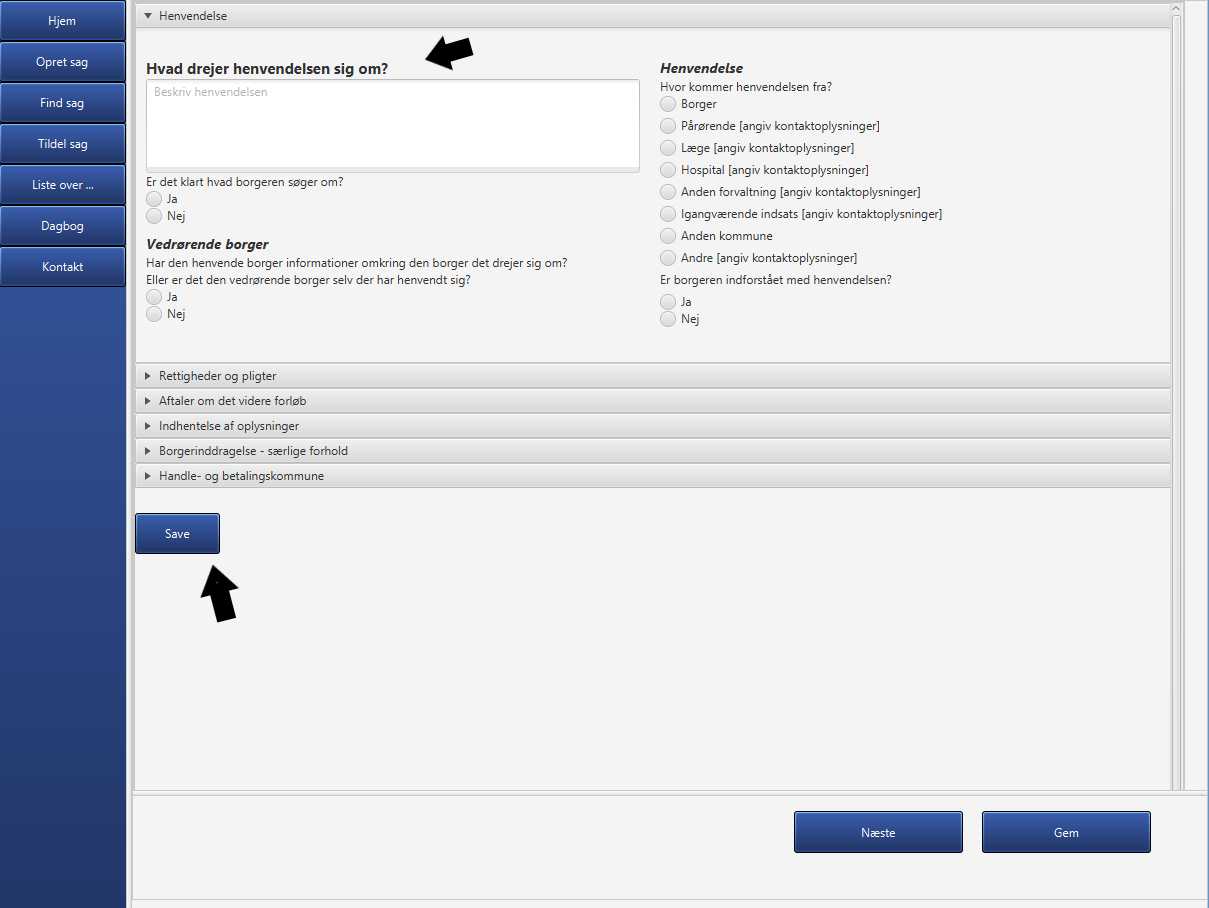
\includegraphics[width = \linewidth]{./PNG/brugervejledning/figur4.PNG} 
  \caption{}  
  \label{bru:f4}
\end{figure}
\newpage
I sagsåbningsformularen kan der skrives oplysninger omkring den henvende borger samt den vedrørende borger. (se figur \ref{bru:f5})
\begin{figure}[htb!]
  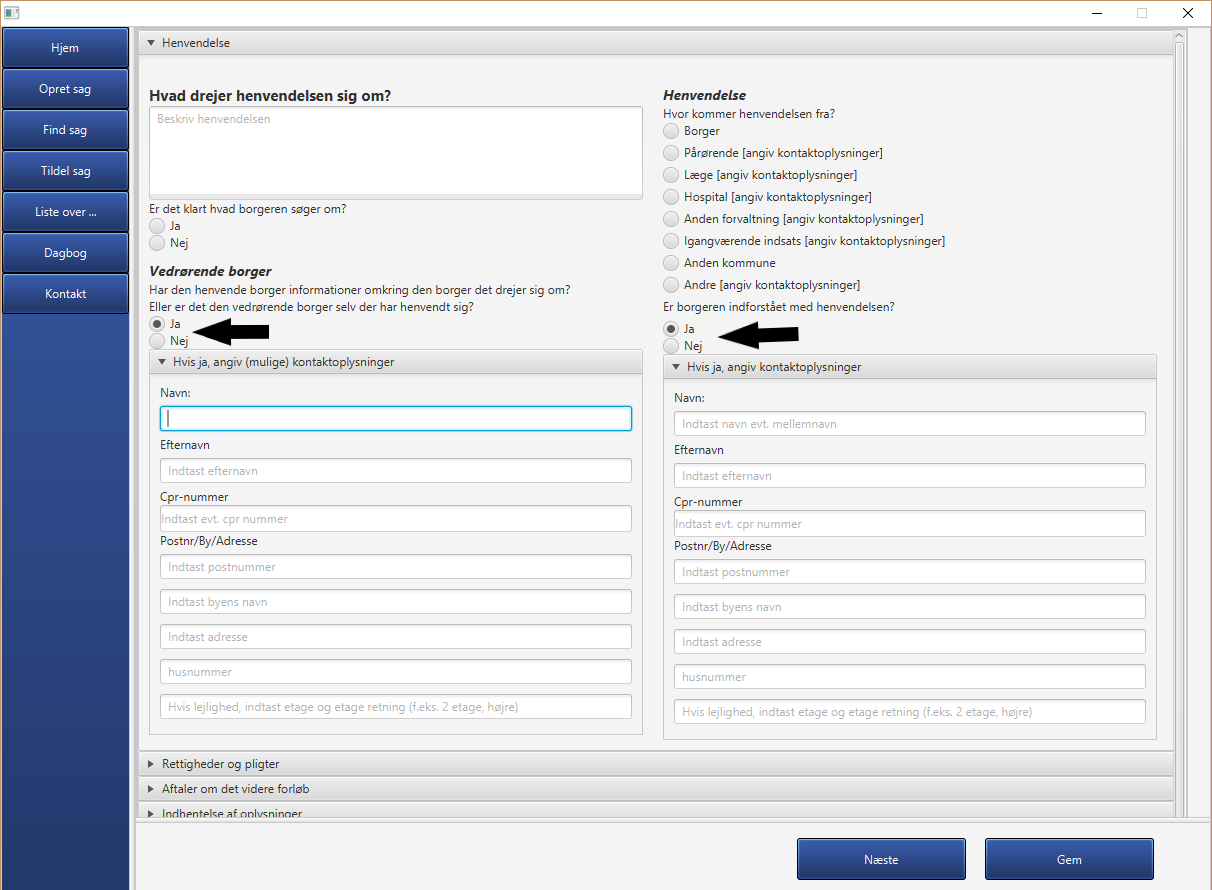
\includegraphics[width = \linewidth]{./PNG/brugervejledning/figur5.PNG} 
  \caption{}  
  \label{bru:f5}
\end{figure}\newpage
Før en ydelse kan blive valgt, skal borgeren være bekendt med hvad han/hun søger om. Hvis ja er markeret, bliver en ny fane stillet til rådighed og der kan vælges ydelser. (se figur \ref{bru:f6})
\begin{figure}[htb!]
  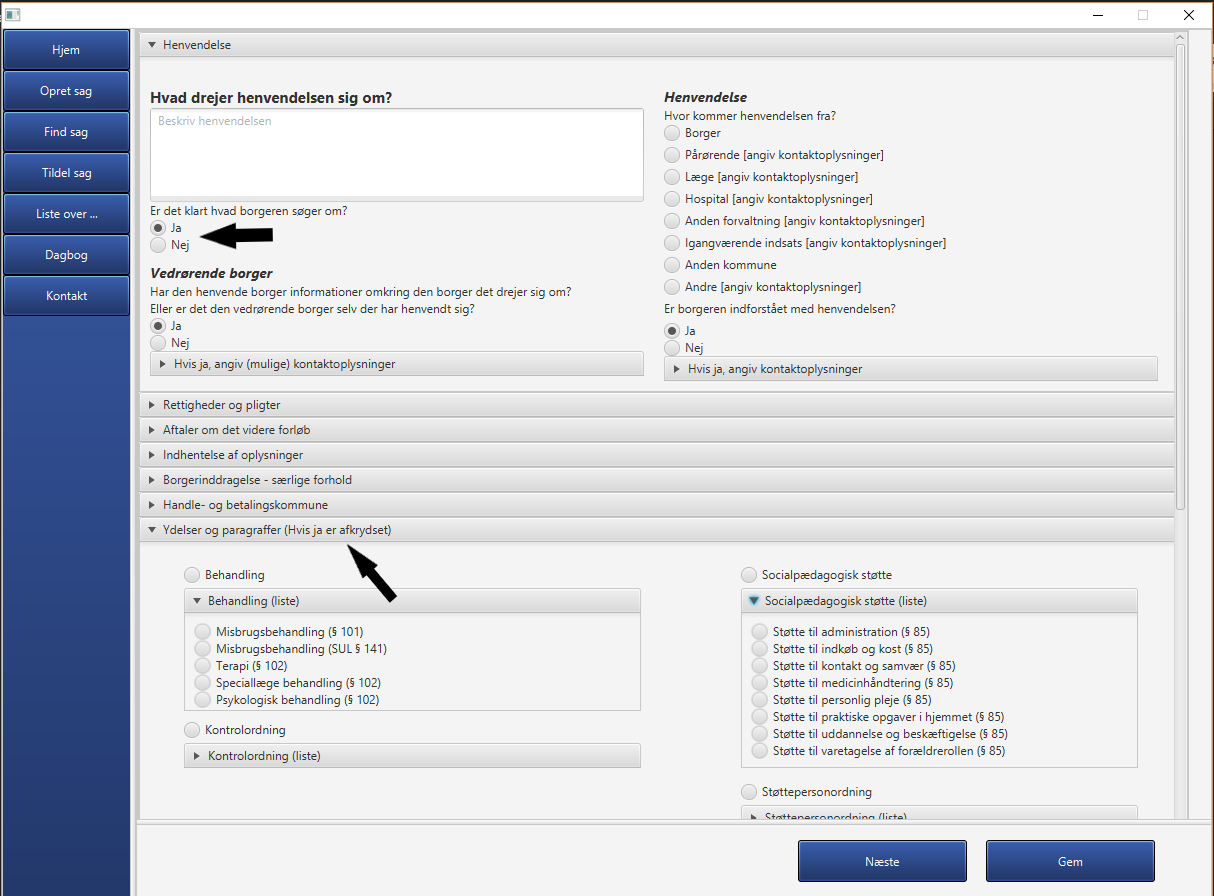
\includegraphics[width = \linewidth]{./PNG/brugervejledning/figur6.PNG} 
  \caption{}  
  \label{bru:f6}
\end{figure}\newpage
Der kan også vælges andre elementer såsom ”aftaler om det videre forløb” eller ”rettigheder og pligter”. Det eneste der skal gøres for at få de elementer frem er ved at folde dem ud ved at klikke på den vandrette lille pil ved siden af teksten til venstre. (se figur \ref{bru:f7})
\begin{figure}[htb!]
  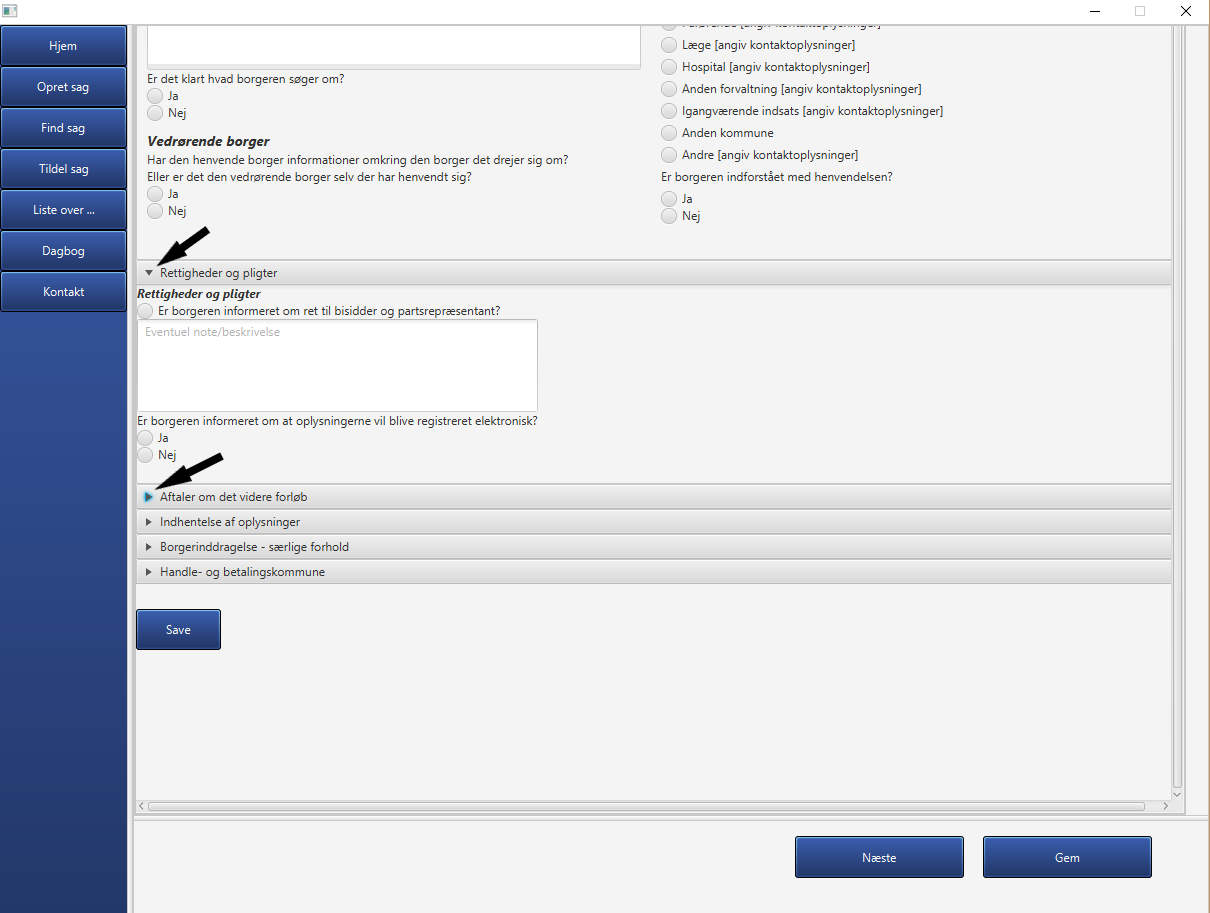
\includegraphics[scale = 0.3]{./PNG/brugervejledning/figur7.PNG} 
  \caption{}  
  \label{bru:f7}
\end{figure}\newpage
Når der er blevet fortaget de nødvendige ændringer, kan sagen gemmes ved at trykke på ”save” knappen. Nu kan der fortsættes med sagsudredningen ved at trykke på ”næste” knappen og der vil blive vist en sagsudredningsformular. I sagsudrednings formularen kan der ligesom i sagsåbningensformularen, udvides faner som har forskellige felter der kan udfyldes. Når man er færdig trykker man på den lille ”gem” knap og herefter trykkes der på den store ”gem” knap”, der gemmer hele dokumentet i systemet. Se figur \ref{bru:f8}
\begin{figure}[htb!]
  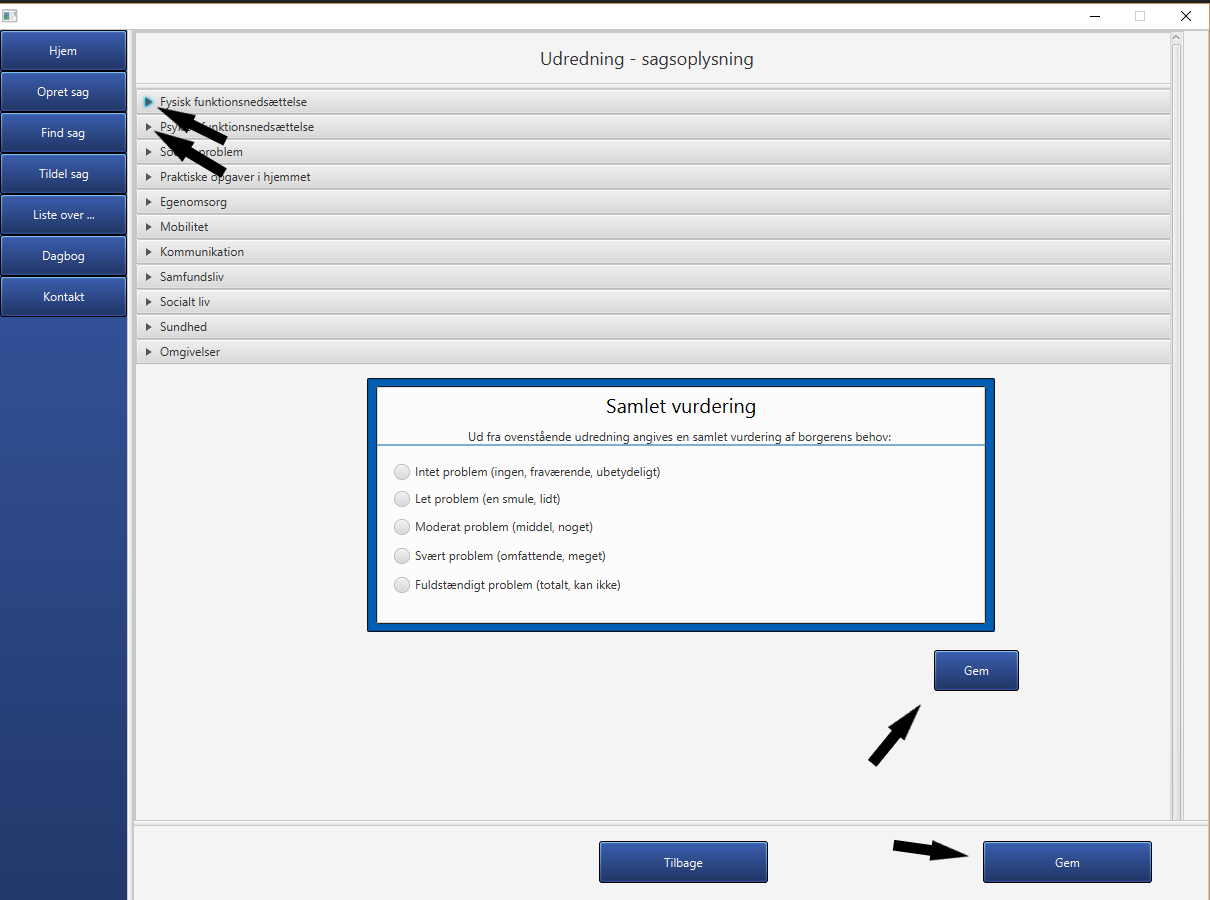
\includegraphics[scale = 0.3]{./PNG/brugervejledning/figur8.PNG} 
  \caption{}  
  \label{bru:f8}
\end{figure}\newpage
Man kan også søge på en borger (se figur \ref{bru:f9}) hvor der kan søges på fire forskellige kritierier og dermed kan man søge de sager frem som en borger er tilknyttet og man får en oversigt vist i det store oversigtsvindue. Ydermere kan der også vælges at søge på et sagsnummer ved at skrive nummert på sagen og herefter trykke på knappen ”søg”. (se figur \ref{bru:f10}) 
\begin{figure}[htb!]
  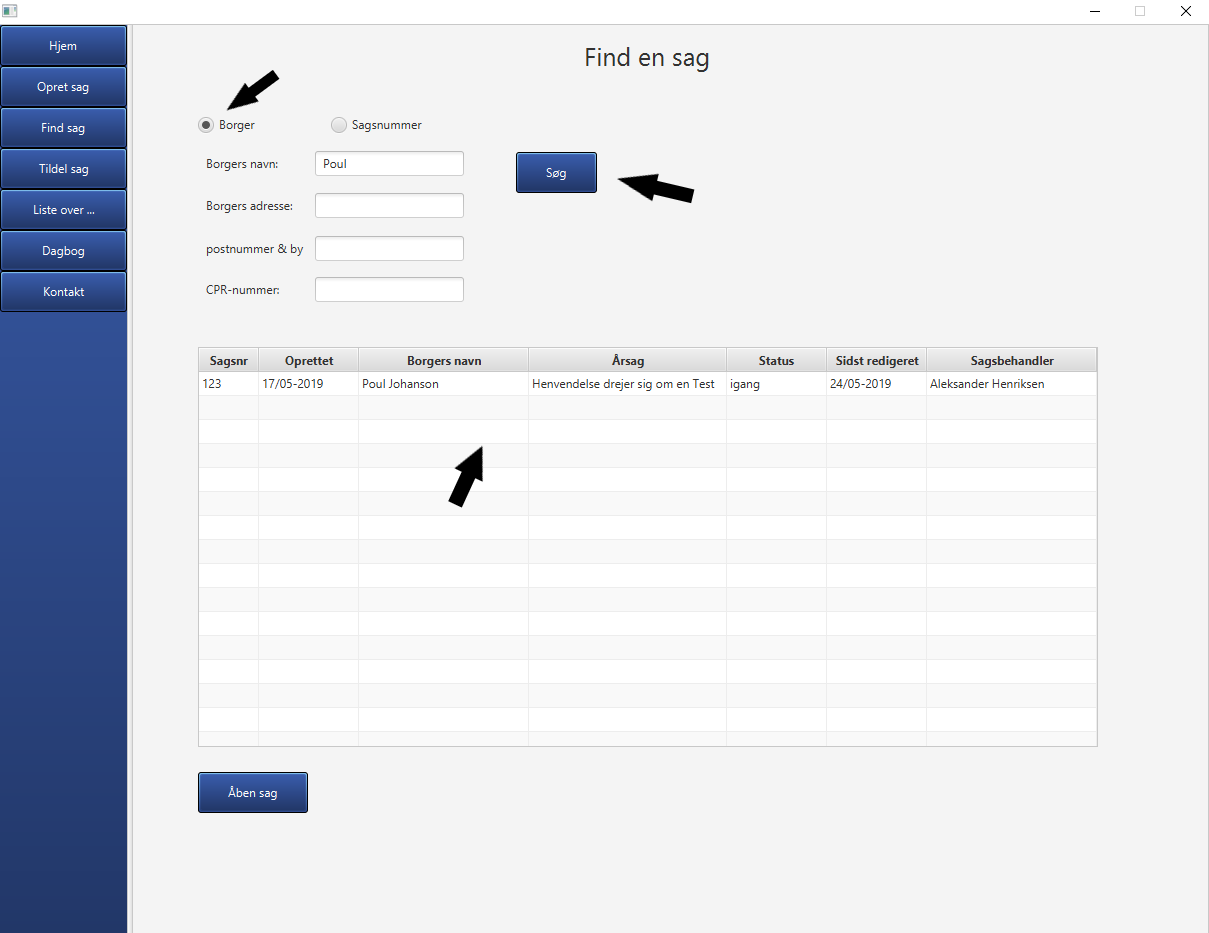
\includegraphics[scale = 0.3]{./PNG/brugervejledning/figur9.PNG} 
  \caption{}  
  \label{bru:f9}
\end{figure}
\begin{figure}[htb!]
  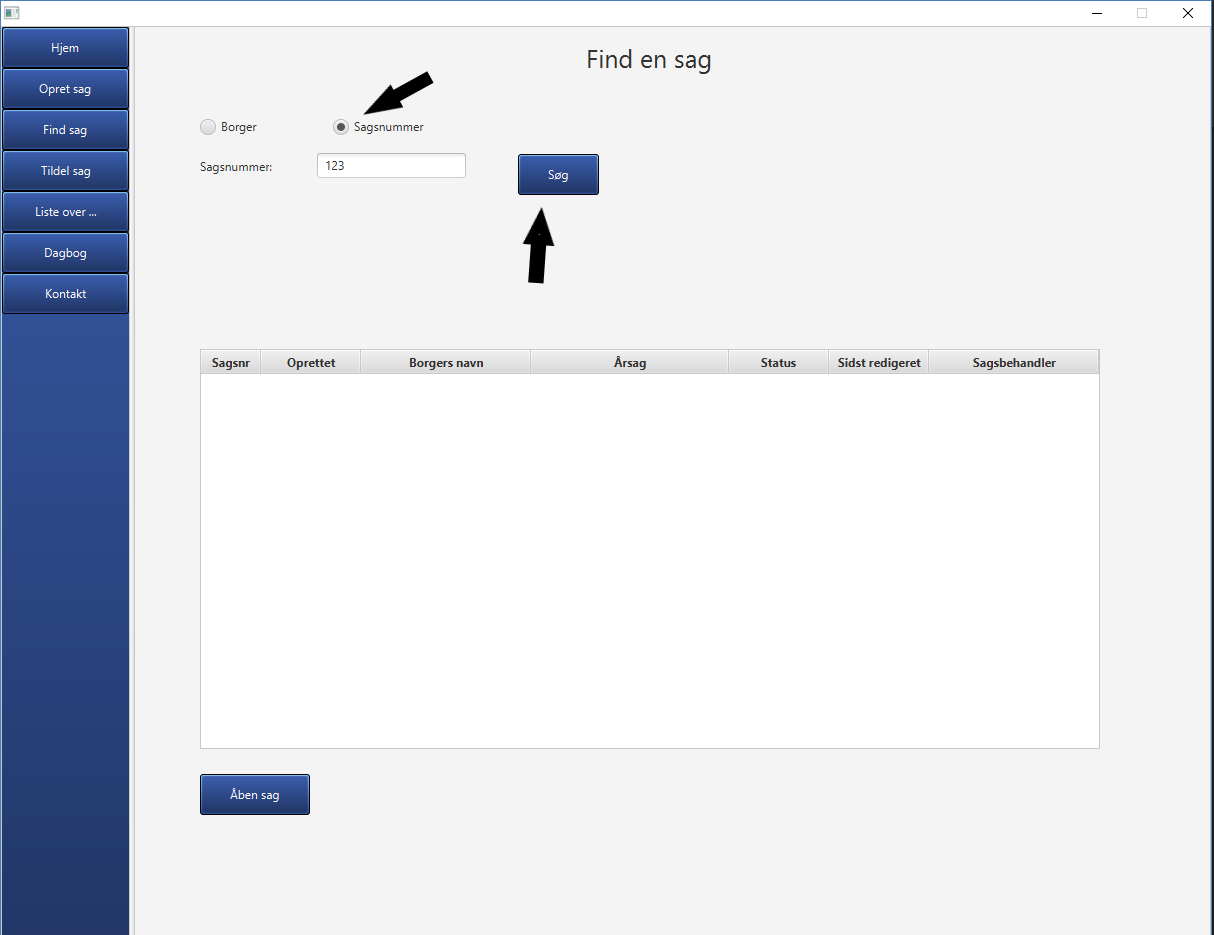
\includegraphics[scale = 0.3]{./PNG/brugervejledning/figur10.PNG} 
  \caption{}  
  \label{bru:f10}
\end{figure}
\newpage
Udover det er der 4 andre knapper, ”tildel sag”, ”liste over sager”, ”dagbog” og ”kontakt” som ikke er blevet implementeret med funktionalitet og kan derfor ikke benyttes (klikkes på). (se figur \ref{bru:f11})\\
\begin{figure}[htb!]
  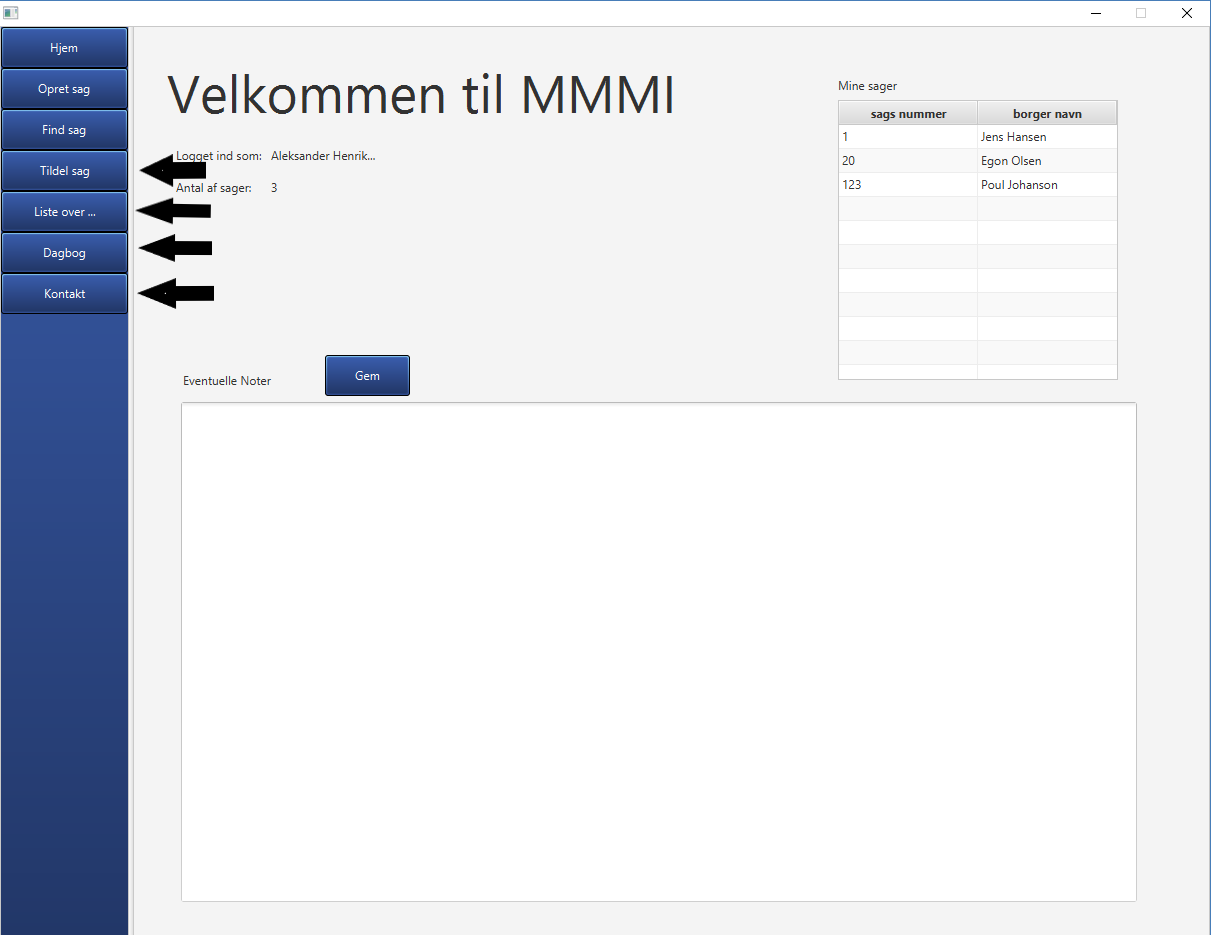
\includegraphics[scale = 0.3]{./PNG/brugervejledning/figur11.PNG} 
  \caption{}  
  \label{bru:f11}
\end{figure}
For at logge ud igen skal vinduet bare lukkes ned ved at trykke på det røde kryds i MMMI vinduet i øverste højre hjørne. Hvis man ønsker at logge ind igen skal man gøre som i starten i brugervejledningen.\\
\newpage